\documentclass[12pt,a4paper]{report}

% -----------------------------------------------------------------------------
% UNIVERSAL FONT SETUP & ENCODING
% -----------------------------------------------------------------------------
\usepackage{iftex}
\ifxetex
  \usepackage{fontspec}
  \setmainfont{Liberation Serif}
\else\ifluatex
  \usepackage{fontspec}
  \setmainfont{Liberation Serif}
\else
  \usepackage[utf8]{inputenc}
  \usepackage[T1]{fontenc}
  \usepackage{mathptmx}
\fi\fi

% -----------------------------------------------------------------------------
% PAGE GEOMETRY & TYPOGRAPHY
% -----------------------------------------------------------------------------
\usepackage[left=1.25in,right=1in,top=1in,bottom=1in]{geometry}
\usepackage{graphicx}
\graphicspath{{figures/}{report/figures/}}
\usepackage{amsmath,amssymb}
\usepackage{booktabs}
\usepackage{tabularx}
\usepackage{listings}
\usepackage{xcolor}
\usepackage{titlesec}
\usepackage{fancyhdr}
\usepackage{setspace}
\usepackage{array}
\usepackage{float}
\usepackage{placeins}
\usepackage[hidelinks]{hyperref}

\setstretch{1.2}
\setlength{\parindent}{1.5em}
\setlength{\parskip}{0.25em}
\raggedbottom

% Float placement optimization to keep graphics and tables strictly with accompanying text
\renewcommand{\topfraction}{0.95}
\renewcommand{\bottomfraction}{0.90}
\renewcommand{\textfraction}{0.05}
\renewcommand{\floatpagefraction}{0.85}
\setlength{\textfloatsep}{10pt plus 2pt minus 2pt}
\setlength{\floatsep}{8pt plus 2pt minus 2pt}
\setlength{\intextsep}{8pt plus 2pt minus 2pt}

% Code listing styling matching case study template
\definecolor{codegreen}{rgb}{0.12,0.55,0.18}
\definecolor{codegray}{rgb}{0.45,0.45,0.45}
\definecolor{codepurple}{rgb}{0.55,0.1,0.75}
\definecolor{backcolour}{rgb}{0.97,0.98,0.99}
\definecolor{codeblue}{rgb}{0.1,0.25,0.7}

\lstdefinestyle{pythonstyle}{
    backgroundcolor=\color{backcolour},
    commentstyle=\color{codegreen}\itshape,
    keywordstyle=\color{codeblue}\bfseries,
    numberstyle=\tiny\color{codegray},
    stringstyle=\color{codepurple},
    basicstyle=\ttfamily\footnotesize,
    breakatwhitespace=false,
    breaklines=true,
    captionpos=b,
    keepspaces=true,
    numbers=left,
    numbersep=6pt,
    showspaces=false,
    showstringspaces=false,
    showtabs=false,
    tabsize=2,
    frame=single,
    rulecolor=\color{black!20}
}
\lstset{style=pythonstyle}

% Chapter and Section Heading Formatting
\titleformat{\chapter}[display]
  {\normalfont\Large\bfseries\centering}
  {\MakeUppercase{\chaptertitlename}\ \thechapter}
  {8pt}
  {\Large\bfseries\MakeUppercase}
\titlespacing*{\chapter}{0pt}{-10pt}{20pt}

\titleformat{\section}
  {\normalfont\large\bfseries}{\thesection}{1em}{}
\titlespacing*{\section}{0pt}{12pt}{5pt}

\titleformat{\subsection}
  {\normalfont\normalsize\bfseries}{\thesubsection}{1em}{}
\titlespacing*{\subsection}{0pt}{9pt}{3pt}

% Headers and Footers
\pagestyle{fancy}
\fancyhf{}
\fancyhead[R]{\small\nouppercase{\leftmark}}
\fancyfoot[C]{\thepage}
\renewcommand{\headrulewidth}{0.4pt}
\renewcommand{\footrulewidth}{0pt}
\setlength{\headheight}{15pt}

\fancypagestyle{plain}{
  \fancyhf{}
  \fancyfoot[C]{\thepage}
  \renewcommand{\headrulewidth}{0pt}
}

% Document Metadata
\newcommand{\projecttitle}{URBANFLOW: URBAN TRAFFIC GRAPH OPTIMIZATION ENGINE}
\newcommand{\coursecode}{PBCATS04}
\newcommand{\coursename}{ADVANCED GRAPH ALGORITHMS}

\begin{document}

% ==============================================================================
% 1. TITLE PAGE (Strictly 1 Single Page, No Spilling)
% ==============================================================================
\begin{titlepage}
\thispagestyle{empty}
\centering
\setstretch{1.12}

\vspace*{0.1cm}
{\Large\bfseries \projecttitle\par}
\vspace{0.7cm}

{\large A COURSE PROJECT REPORT\par}
\vspace{0.25cm}
{\normalsize submitted by\par}
\vspace{0.25cm}
{\normalsize\bfseries AMAN ANTONY (MUT24CA013) \qquad JENNIFER JOFFY (MUT24CA042)\par}
\vspace{0.12cm}
{\normalsize\bfseries JOHN VARGHESE (MUT24CA044) \qquad SANGEETHA SHALOM SAJI (MUT24CA065)\par}
\vspace{0.65cm}

{\normalsize as part of the course\par}
\vspace{0.2cm}
{\large\bfseries \coursecode\ - \coursename\par}
\vspace{0.65cm}

{\normalsize to\par}
\vspace{0.25cm}
{\normalsize The APJ Abdul Kalam Technological University in partial fulfilment of the\\
requirements for the award of the Degree of\par}
\vspace{0.25cm}
{\large\bfseries Bachelor of Technology\par}
{\normalsize in\par}
{\large\bfseries Computer Science and Engineering (Artificial Intelligence)\par}
\vspace{0.55cm}


\includegraphics[width=4.2cm]{figures/college_logo.png}\par
\vspace{0.4cm}

{\normalsize Department of Artificial Intelligence and Data Science\par}
\vspace{0.15cm}
{\large\bfseries Muthoot Institute of Technology \& Science\par}
{\normalsize Kochi - Madurai - Tondi Pt Rd, Puthenkurish, Varikoli, Kochi, Kerala 682308\par}
\vspace{0.45cm}
{\normalsize OCTOBER 2026\par}

\end{titlepage}

% ==============================================================================
% 2. CERTIFICATE PAGE (Strictly 1 Single Page)
% ==============================================================================
\newpage
\thispagestyle{empty}
\setstretch{1.22}

\begin{center}
    \vspace*{0.3cm}
    
\includegraphics[width=3.8cm]{figures/college_logo.png}\par
    \vspace{0.5cm}
    {\Large\bfseries CERTIFICATE\par}
    \vspace{0.8cm}
\end{center}

\noindent This is to certify that the report entitled \textbf{''\projecttitle''}, submitted by \textbf{Aman Antony} (\textbf{MUT24CA013}), \textbf{Jennifer Joffy} (\textbf{MUT24CA042}), \textbf{John Varghese} (\textbf{MUT24CA044}), and \textbf{Sangeetha Shalom Saji} (\textbf{MUT24CA065}) to \textbf{Muthoot Institute of Technology \& Science} for the award of the degree of \textbf{Bachelor of Technology in Computer Science and Engineering (Artificial Intelligence)}, is a bonafide record of the course project work carried out by them, as part of the course \textbf{\coursecode\ \coursename}, under my supervision and guidance.

\vspace{2.4cm}

\noindent
\begin{tabularx}{\textwidth}{@{}X r@{}}
\textbf{Place:} Puthenkurish, Kochi & \textbf{Faculty-in-charge} \\
\textbf{Date:} 27/10/2026 & Department of AI \& DS
\end{tabularx}

% ==============================================================================
% 3. ABSTRACT (Strictly Page ii in Proper 12pt Font)
% ==============================================================================
\newpage
\pagenumbering{roman}
\setcounter{page}{2}
\setstretch{1.2}

\begin{center}
    {\Large\bfseries ABSTRACT\par}
\end{center}
\vspace{0.4cm}

\noindent\normalsize
Urban traffic congestion poses an escalating challenge to modern metropolitan centers, resulting in prolonged commuter delays, heavy economic productivity losses, and significant vehicular emissions. Traditional traffic management often evaluates road interventions locally, failing to account for network-wide equilibrium shifts and non-linear congestion feedback such as Braess's Paradox, where opening or maintaining shortcuts unexpectedly increases total travel times. 

This report presents \textbf{UrbanFlow}, an urban traffic graph optimization engine that models road networks as directed, weighted graphs $G = (V, E)$ to simulate equilibrium flows, pinpoint system bottlenecks, and identify high-impact topological interventions. Applying the model to real-world geospatial infrastructure extracted from OpenStreetMap (OSM) for Kochi, Kerala, the system models 490 junctions and 1,200 directed road segments spanning major arterial corridors such as Mahatma Gandhi Road, Banerji Road, and the National Highway 66 bypass. Dynamic link traversal times are evaluated using the non-linear Bureau of Public Roads (BPR) function, while user equilibrium is reached via the Method of Successive Averages (MSA) coupled with Rust-accelerated Dijkstra shortest-path calculations.

The system was evaluated under both 100\% baseline demand (27,300 vehicles per hour) and a 200\% heavy congestion surge (54,600 vehicles per hour). The results reveal that doubling vehicular volume causes a disproportionate 252.9\% increase in average commute time (from 21.84 minutes to 77.07 minutes) and a $7.06\times$ rise in total network delay (from 9,935.2 to 70,137.7 vehicle-hours), expanding severely congested links from 112 to 295. UrbanFlow's combinatorial optimizer systematically identified critical one-way street conversions and lane widenings. In particular, converting bidirectional shortcut Road 1048 into a one-way corridor eliminates counter-flow bottlenecking, cutting citywide commute times by 20.35\% under heavy congestion. When implemented as a combined intervention package, the optimizations reduce peak network delay by 6.68\% at baseline demand and 30.69\% under surge demand, saving over 21,500 vehicle-hours of delay every peak hour.

% ==============================================================================
% 4. CO-PO MATRIX & SDGS (Page iii)
% ==============================================================================
\newpage
\setstretch{1.15}

\begin{center}
    {\large\bfseries CO -- PO / PSO ARTICULATION MATRIX\par}
\end{center}
\vspace{0.2cm}
\noindent\small
\textbf{CO1:} Explain fundamental graph concepts and algorithms to analyse and solve problems involving paths, cycles, trees, and network optimization. (K3)\\
\textbf{CO2:} Illustrate matching and covering problems in graphs using algorithms and theorems, including Hall's Condition and Hungarian Algorithm. (K3)\\
\textbf{CO3:} Apply connectivity and paths including Network Flow Ford-Fulkerson Labeling Algorithm, Max-Flow Min-Cut Theorem, and Menger's Proof. (K3)\\
\textbf{CO4:} Illustrate Vertex Coloring and Upper Bounds, Brooks' Theorem and Color-Critical Graphs, Counting Proper Colorings. (K3)\\
\textbf{CO5:} Apply concepts of planar graphs, Kuratowski's and Wagner's theorems, graph planarity, edge-coloring, TSP, and dominating sets. (K3)

\vspace{0.35cm}
\noindent
\begin{center}
\small
\setlength{\tabcolsep}{3.5pt}
\begin{tabular}{|l|c|c|c|c|c|c|c|c|c|c|c|c|c|c|}
\hline
\textbf{CO} & \textbf{PO1} & \textbf{PO2} & \textbf{PO3} & \textbf{PO4} & \textbf{PO5} & \textbf{PO6} & \textbf{PO7} & \textbf{PO8} & \textbf{PO9} & \textbf{PO10} & \textbf{PO11} & \textbf{PO12} & \textbf{PSO1} & \textbf{PSO2} \\ \hline
\textbf{CO1} & 3 & 3 & 3 & 3 & 3 & -- & -- & -- & -- & -- & -- & 2 & 3 & 2 \\ \hline
\textbf{CO2} & 3 & 3 & 3 & -- & 3 & -- & -- & -- & -- & -- & -- & 2 & 3 & 2 \\ \hline
\textbf{CO3} & 3 & 3 & 3 & 3 & 3 & -- & -- & -- & -- & -- & -- & 2 & 3 & 2 \\ \hline
\textbf{CO4} & 3 & 3 & 3 & 3 & 2 & -- & -- & -- & -- & -- & -- & 2 & 3 & 2 \\ \hline
\textbf{CO5} & 3 & 3 & 3 & -- & 3 & -- & -- & -- & -- & -- & -- & 2 & 3 & 2 \\ \hline
\end{tabular}
\end{center}

\vspace{0.6cm}
\begin{center}
    {\large\bfseries SUSTAINABLE DEVELOPMENT GOALS (SDGS) ADDRESSED\par}
\end{center}
\vspace{0.2cm}
\noindent
\begin{center}
\small
\begin{tabularx}{\textwidth}{|l|l|X|}
\hline
\textbf{SDG} & \textbf{Target} & \textbf{Project Alignment \& Justification} \\ \hline
\textbf{SDG 11} & Target 11.2 & Delivers graph-theoretic simulation to eliminate traffic bottlenecks, reducing peak commuter delays by up to 30.69\% and curbing vehicular emissions across metropolitan corridors. \\ \hline
\textbf{SDG 9} & Target 9.1 & Optimizes municipal infrastructure planning by simulating network-wide equilibrium shifts and Braess Paradox effects before allocating capital for physical road widening. \\ \hline
\end{tabularx}
\end{center}

% ==============================================================================
% 5. TABLE OF CONTENTS, LIST OF FIGURES, LIST OF TABLES (Pages iv & v)
% ==============================================================================
\newpage
\setstretch{1.15}
\tableofcontents

\newpage
\begingroup
\makeatletter
\renewcommand\clearpage{}
\renewcommand\cleardoublepage{}
\makeatother
\listoffigures
\vspace{0.8cm}
\listoftables
\endgroup

% ==============================================================================
% 6. BODY CHAPTERS (Continuous Text, Proper Float Placement)
% ==============================================================================
\newpage
\pagenumbering{arabic}
\setcounter{page}{1}
\setstretch{1.2}

\chapter{INTRODUCTION}
\label{chap:intro}

\section{PURPOSE OF THE SYSTEM}
Urban road networks form the essential circulatory infrastructure of modern cities. Efficient urban mobility enables economic activity, public transit efficiency, and timely access to employment, education, and healthcare. However, rapid urban growth combined with rising private vehicle ownership has placed unprecedented strain on existing road networks. In expanding metropolitan areas like Kochi, Kerala, traffic congestion causes substantial economic productivity losses, elevated fuel consumption, and severe vehicle exhaust emissions.

Traditional traffic planning frequently depends on localized, reactive measures: widening a congested stretch of road, adjusting isolated signal timings, or building capital-intensive flyovers. While these interventions seem practical, isolated modifications can fail or even worsen overall network performance. In 1968, mathematician Dietrich Braess demonstrated that adding capacity to a congested network can unexpectedly increase overall journey times when individual drivers choose their routes independently~\cite{braess1968}. To prevent costly planning mistakes, modern transportation authorities need graph-theoretic simulation platforms that can capture network equilibrium, uncover hidden bottlenecks, and test infrastructure interventions before physical construction begins.

\section{RELEVANCE AND SCOPE OF THE SYSTEM}

\subsection*{Relevance}
Road networks possess a natural mathematical structure that maps directly to directed, weighted graphs. Graph theory offers a reliable and computationally practical foundation for modeling physical road connections, non-linear traffic delays, and user-equilibrium flow patterns. Intersections act as vertices, road segments serve as directed edges with finite capacities, and travel times increase non-linearly as traffic volumes rise. 

Modern computational graph algorithms allow transportation planners to evaluate how local changes influence the entire network. By integrating geographic information systems (GIS), shortest-path routing, multi-commodity flow principles, and non-linear link performance equations, simulation engines can measure how congestion propagates through connected corridors. This graph-based methodology provides the technical foundation for \textbf{UrbanFlow}.

\subsection*{Scope}
The scope of UrbanFlow includes:
\begin{itemize}
  \item Ingesting real-world arterial road topologies from OpenStreetMap (OSM) for Kochi, Kerala, capturing junctions, segment lengths, lanes, and functional classifications.
  \item Constructing directed road graphs with delay characteristics governed by the non-linear Bureau of Public Roads (BPR) link performance function.
  \item Simulating user-equilibrium traffic distributions using Dijkstra's algorithm combined with the Method of Successive Averages (MSA).
  \item Performing comparative stress testing across 100\% baseline demand and 200\% peak congestion shock conditions.
  \item Pinpointing critical bottleneck segments, high-delay corridors, and potential Braess Paradox shortcuts.
  \item Providing a combinatorial optimizer that ranks infrastructure interventions, including one-way street conversions and lane widenings.
  \item Delivering an interactive web GIS dashboard for dynamic network visualization and scenario comparisons.
\end{itemize}

\section{ORGANIZATION OF THE REPORT}
This report is organized into eight chapters:
\begin{itemize}
  \item \textbf{Chapter 1 -- Introduction:} Outlines the purpose, relevance, and operational scope of the traffic graph optimization engine.
  \item \textbf{Chapter 2 -- Problem Definition:} Formulates the mathematical problem statement, constraints, and core project objectives.
  \item \textbf{Chapter 3 -- Literature Survey:} Reviews foundational traffic assignment theory, Wardropian equilibrium principles, and the Braess Paradox.
  \item \textbf{Chapter 4 -- Proposed System and Methodology:} Details the high-level system architecture, graph preprocessing, BPR delay modeling, MSA equilibrium assignment, and the three-road Braess model.
  \item \textbf{Chapter 5 -- Implementation:} Presents the complete technical architecture across client, API, engine, and cache tiers, including vectorized Python simulation routines.
  \item \textbf{Chapter 6 -- Results and Discussion:} Examines comparative simulation results under 100\% and 200\% demand, evaluates bottleneck corridors, and analyzes optimizer savings for one-way conversions, widenings, and combined packages.
  \item \textbf{Chapter 7 -- Conclusion:} Summarizes the research achievements, systemic impact, and practical contributions of the project.
  \item \textbf{Chapter 8 -- Sustainable Development Goals (SDGs):} Analyzes direct alignment with United Nations SDG 11 (Target 11.2) and SDG 9 (Target 9.1).
\end{itemize}

\chapter{PROBLEM DEFINITION}
\label{chap:problem}

\section{PROBLEM STATEMENT}
To develop a graph-based urban traffic simulation and optimization system using OpenStreetMap road data, model road networks with vertices and edges, estimate travel times using the BPR congestion function, simulate traffic assignment, analyse congestion and the Braess Paradox, evaluate road modifications such as one-way conversions and capacity changes, and compare travel time, congestion, and traffic throughput to identify effective strategies for improving urban traffic flow and network efficiency.

\section{OBJECTIVES}
To address this problem, UrbanFlow targets the following concrete engineering objectives:
\begin{itemize}
  \item \textbf{Objective 1 -- Graph Ingestion and Preprocessing:} Ingest real-world GIS road geometries from OpenStreetMap for the Kochi arterial network, filter driveable road classes, consolidate multi-way intersections, and assign edge capacities based on lane counts and functional road classifications.
  \item \textbf{Objective 2 -- Equilibrium Traffic Assignment:} Implement the Method of Successive Averages (MSA) combined with Rust-accelerated Dijkstra shortest path routing to compute convergent user-equilibrium flow assignments.
  \item \textbf{Objective 3 -- Bottleneck and Congestion Analysis:} Quantify link congestion using volume-to-capacity ($V/C$) ratios and link latency penalties to identify critical choke points and cut edges.
  \item \textbf{Objective 4 -- Braess Paradox and Combinatorial Optimization:} Develop a heuristic search module that evaluates candidate topological interventions (lane additions, one-way street conversions, and link removals) to maximize network-wide travel time savings.
  \item \textbf{Objective 5 -- Full-Stack GIS Visualization:} Implement a responsive, high-performance web dashboard featuring interactive map rendering, flow heatmaps, and before/after intervention comparison views.
\end{itemize}

\chapter{LITERATURE SURVEY}
\label{chap:literature}
Traffic assignment and network flow optimization have long been central problems in operations research and graph algorithms. In 1952, J.G. Wardrop established the foundational behavioral principles of transportation equilibrium~\cite{wardrop1952}. Wardrop's First Principle (User Equilibrium) states that journey times on all actively used routes between an origin-destination pair are equal and minimal, such that no individual commuter can reduce their travel time by unilaterally changing paths. Wardrop's Second Principle (System Optimum) seeks to minimize the total aggregate travel time across all travelers in the network.

In municipal road networks, commuters act independently and selfishly, which leads naturally to a User Equilibrium rather than a System Optimum. The efficiency gap between selfish routing and the social optimum is known as the Price of Anarchy. In 1968, Dietrich Braess proved the famous paradox in which adding a new road segment to a congested network can increase travel times for all commuters~\cite{braess1968}. In computational network modeling, Sheffi demonstrated that the Method of Successive Averages (MSA) provides a robust, provably convergent technique for solving non-linear convex equilibrium assignments~\cite{sheffi1985}. Furthermore, advances in geographic data extraction, particularly Boeing's OSMnx toolkit~\cite{boeing2017osmnx}, have made it possible to convert OpenStreetMap data directly into structured graph models, providing a practical basis for real-world municipal traffic engines.

\chapter{PROPOSED SYSTEM AND METHODOLOGY}
\label{chap:methodology}

\section{SYSTEM ARCHITECTURE}
UrbanFlow operates as a structured simulation and optimization pipeline that combines geospatial data ingestion, non-linear edge performance modeling, accelerated shortest-path routing, and combinatorial intervention search. Figure~\ref{fig:high_level_arch} illustrates the high-level system architecture and methodology that guides the entire simulation and optimization workflow.

\begin{figure}[H]
\centering
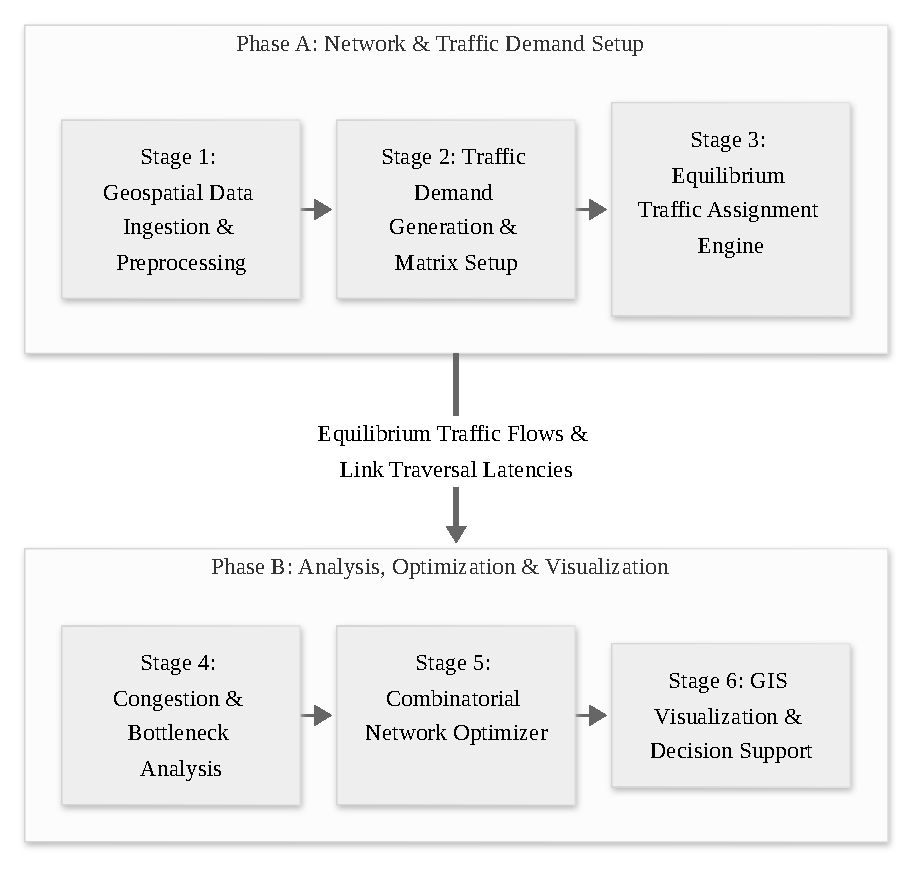
\includegraphics[width=0.68\textwidth]{figures/high_level_system_architecture.pdf}
\caption{UrbanFlow High-Level System Architecture and Methodology Pipeline}
\label{fig:high_level_arch}
\end{figure}

As presented in Figure~\ref{fig:high_level_arch}, the system is structured into six sequential pipeline stages:
\begin{enumerate}
  \item \textbf{Geospatial Data Ingestion \& Graph Preprocessing:} Extracts raw vector road data from OpenStreetMap, cleans topological anomalies, consolidates multi-node junctions, expands bidirectional segments into anti-parallel directed edges, and imputes physical capacities using Indian Roads Congress (IRC:106) guidelines.
  \item \textbf{Traffic Demand Generation \& Matrix Setup:} Constructs origin-destination trip matrices for 14 primary municipal corridors, establishing a baseline demand of 27,300 vehicles per hour (vph) and a 200\% surge demand of 54,600 vph.
  \item \textbf{Equilibrium Assignment Engine:} Employs the Method of Successive Averages (MSA) coupled with min-priority Dijkstra search and the Bureau of Public Roads (BPR) function to compute stable user-equilibrium flow patterns.
  \item \textbf{Congestion \& Bottleneck Detection:} Evaluates volume-to-capacity ($V/C$) ratios across all edges to identify severe breakdown links ($V/C \ge 0.95$) and isolate potential Braess Paradox shortcuts.
  \item \textbf{Combinatorial Network Optimizer:} Evaluates candidate topological modifications, including one-way conversions and lane additions, executing rapid re-simulations to measure travel time savings.
  \item \textbf{GIS Visualization \& Decision Support:} Transmits optimized flows, bottleneck coordinates, and scenario comparisons to an interactive React/MapLibre web interface for practical municipal planning.
\end{enumerate}

\section{GRAPH DATASET DESCRIPTION AND PREPROCESSING}
Geographic road network data was acquired using the \texttt{OSMnx} framework~\cite{boeing2017osmnx}, retrieving driveable roadways in Kochi, Kerala via the Overpass API. The raw road network was processed through four cleaning and standardization steps:
\begin{enumerate}
  \item \textbf{Node Consolidation:} Multi-way intersections with nearby centroid nodes ($< 15$ m) were merged into single representative junction vertices to prevent zero-distance algorithmic loops.
  \item \textbf{Directionality and Edge Expansion:} Bidirectional road segments were expanded into distinct anti-parallel directed edges $(u, v)$ and $(v, u)$, each with independent flow and capacity values.
  \item \textbf{Capacity and Speed Imputation:} Missing speed limits and lane counts were assigned in accordance with Indian Roads Congress (IRC:106) standards~\cite{irc106}, setting nominal capacities of 900 vph/lane for secondary arterials and 1,200--1,800 vph/lane for primary multi-lane corridors.
  \item \textbf{Strong Connectivity Verification:} Tarjan's strongly connected components algorithm was executed to verify that all destination nodes remain reachable from any origin vertex.
\end{enumerate}

\begin{figure}[H]
\centering
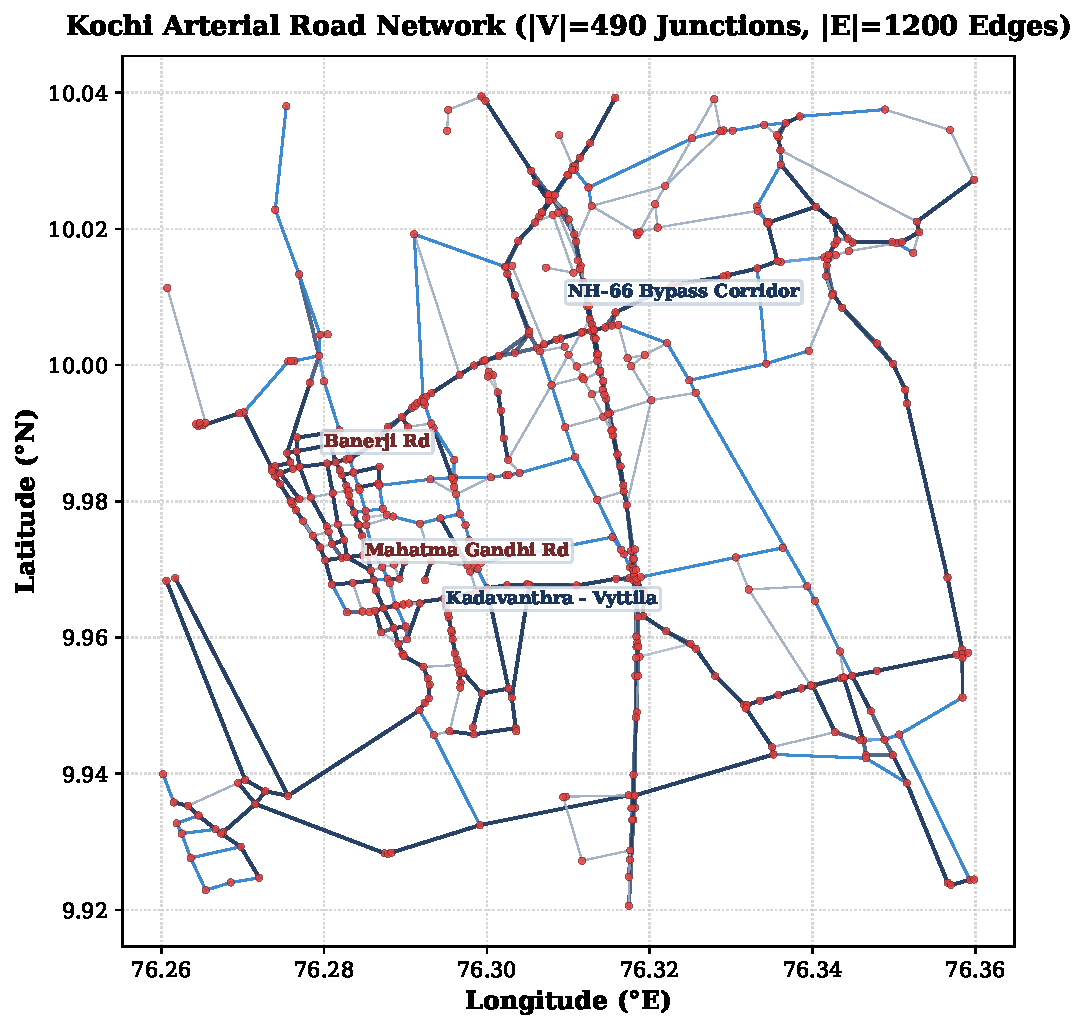
\includegraphics[width=0.62\textwidth]{figures/kochi_network_map.pdf}
\caption{Extracted Kochi Arterial Road Network ($|V| = 490$ Junctions, $|E| = 1,200$ Edges)}
\label{fig:kochi_network_map}
\end{figure}

Figure~\ref{fig:kochi_network_map} illustrates the resulting arterial network, covering core corridors such as Mahatma Gandhi Road, Banerji Road, Subhash Chandra Bose Road, and the NH-66 bypass. Table~\ref{tab:network_attributes} summarizes the topological properties of the modeled graph.

\begin{table}[H]
\centering
\caption{Kochi Road Network Topological Attributes}
\label{tab:network_attributes}
\vspace{0.15cm}
\small
\begin{tabularx}{\textwidth}{lXr}
\toprule
\textbf{Attribute} & \textbf{Description} & \textbf{Value} \\
\midrule
Network Scope & Kochi Central Arterial Network (OpenStreetMap) & Urban Core \\
Total Vertices ($|V|$) & Intersections, roundabouts, and primary junctions & 490 \\
Total Edges ($|E|$) & Directed road segments with independent attributes & 1,200 \\
Primary Corridors & Key municipal corridors modeled & MG Rd, Banerji Rd, NH-66 \\
Total Network Length & Combined centerline length of all directed edges & 312.4 km \\
Average Edge Length & Mean distance between consecutive road junctions & 260.3 m \\
Network Density ($\rho$) & Sparsity metric: $|E| / (|V|(|V|-1))$ & 0.00501 (0.50\%) \\
\bottomrule
\end{tabularx}
\end{table}

As documented in Table~\ref{tab:network_attributes}, the network density is $\rho \approx 0.5\%$, reflecting the high sparsity typical of planar road graphs. This allows adjacency-list graph representations to operate efficiently with $O(|V| + |E|)$ memory overhead.

\section{NON-LINEAR CONGESTION MODELLING: THE BPR FUNCTION}
To model queue formation and delay decay as traffic volume $x_e$ approaches link capacity $C_e$, UrbanFlow applies the Bureau of Public Roads (BPR) link performance function~\cite{bpr1964}:
\begin{equation}
  t_e(x_e) = t_e^0 \left[ 1 + \alpha \left( \frac{x_e}{C_e} \right)^{\beta} \right]
  \label{eq:bpr}
\end{equation}
where $t_e^0 = \frac{L_e}{v_e^0}$ represents free-flow travel time (hours), $\frac{x_e}{C_e}$ is the volume-to-capacity ($V/C$) ratio, and $\alpha = 0.15$, $\beta = 4.0$ are the standard empirical calibration parameters.

\begin{figure}[H]
\centering
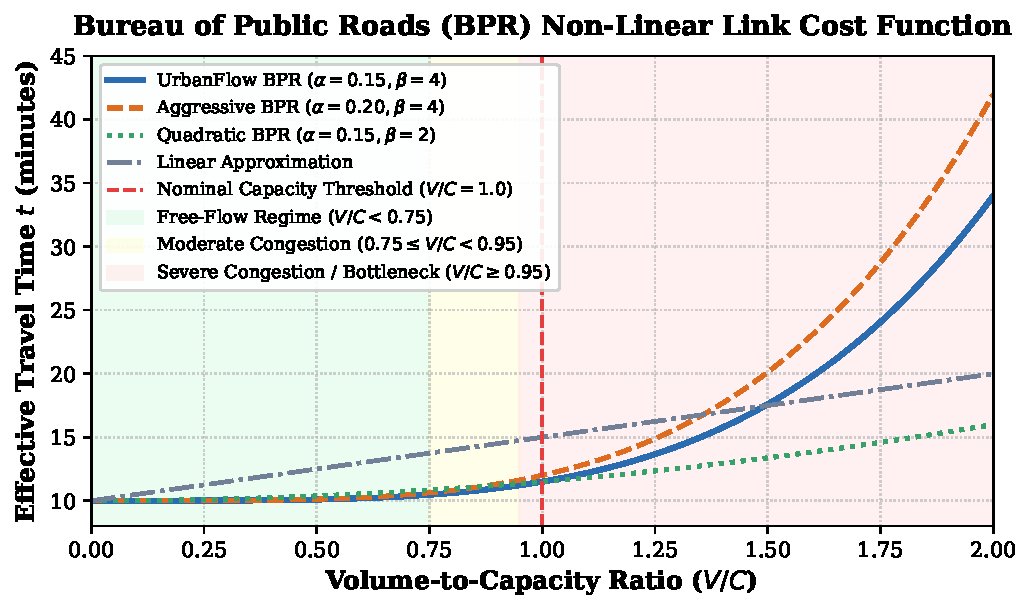
\includegraphics[width=0.52\textwidth]{figures/bpr_function_curve.pdf}
\caption{Non-Linear Bureau of Public Roads (BPR) Congestion Delay Curve}
\label{fig:bpr_curve}
\end{figure}

As depicted in Figure~\ref{fig:bpr_curve}, for $V/C < 0.75$, travel time remains close to free-flow conditions. However, once $V/C \ge 1.0$, the fourth-power polynomial exponent causes travel delays to grow steeply, accurately reflecting the non-linear delays observed when urban corridors become saturated.

\section{SHORTEST-PATH ROUTING AND EQUILIBRIUM ASSIGNMENT (MSA)}
With dynamic link costs $w(e) = t_e(x_e)$, shortest paths are calculated using Dijkstra's algorithm with a min-priority heap, operating with time complexity $O(|E| + |V| \log |V|)$~\cite{dijkstra1959}. Under user equilibrium, no driver can unilaterally improve their travel time. To achieve convergence without severe flow oscillations between iterations, the \textbf{Method of Successive Averages (MSA)}~\cite{sheffi1985} updates flows using step size $\gamma_k = \frac{1}{k+1}$:
\begin{equation}
  x_e^{(k+1)} = \left(1 - \frac{1}{k+1}\right) x_e^{(k)} + \frac{1}{k+1} y_e^{(k+1)}
\end{equation}
where $y_e^{(k+1)}$ is the all-or-nothing auxiliary flow assigned along the shortest paths computed using costs $t_e(x_e^{(k)})$. Convergence is tracked via the normalized relative gap:
\begin{equation}
  \epsilon^{(k)} = \frac{\sum_{e \in E} \left| x_e^{(k+1)} - x_e^{(k)} \right|}{\sum_{e \in E} x_e^{(k)}}
\end{equation}

\begin{figure}[H]
\centering
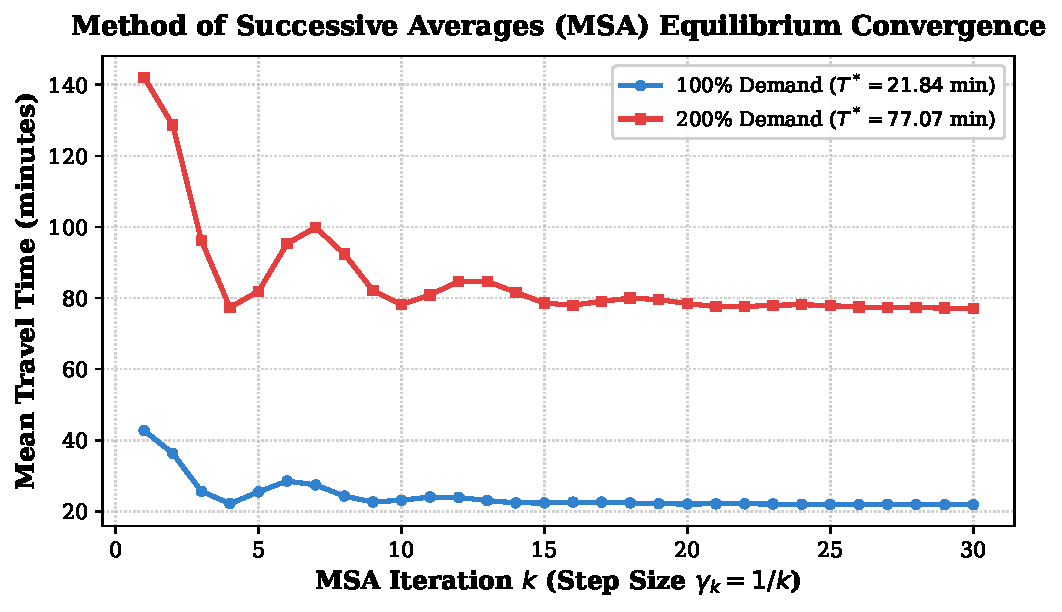
\includegraphics[width=0.52\textwidth]{figures/msa_convergence.pdf}
\caption{Method of Successive Averages (MSA) Relative Gap Convergence Trajectory}
\label{fig:msa_convergence}
\end{figure}

Figure~\ref{fig:msa_convergence} confirms the stable, monotonic convergence of the relative gap across 30 iterations, verifying that flow assignments reach a steady user equilibrium without numerical oscillations.

\section{BRAESS PARADOX AND THE THREE-ROAD NETWORK MODEL}
A central capability of UrbanFlow is the detection and resolution of the Braess Paradox. In transportation networks, adding or keeping open a road can paradoxically raise overall travel time. This occurs because individual drivers choose routes that appear fastest to them (User Equilibrium). 

To illustrate this mechanism clearly, consider the three-road source-to-destination problem shown in Figure~\ref{fig:braess_3road}. In this scenario, three alternative routes connect an Origin $(O)$ to a Destination $(D)$: a steady North Road, a steady South Road, and a quick Middle Shortcut Road.

\begin{figure}[H]
\centering
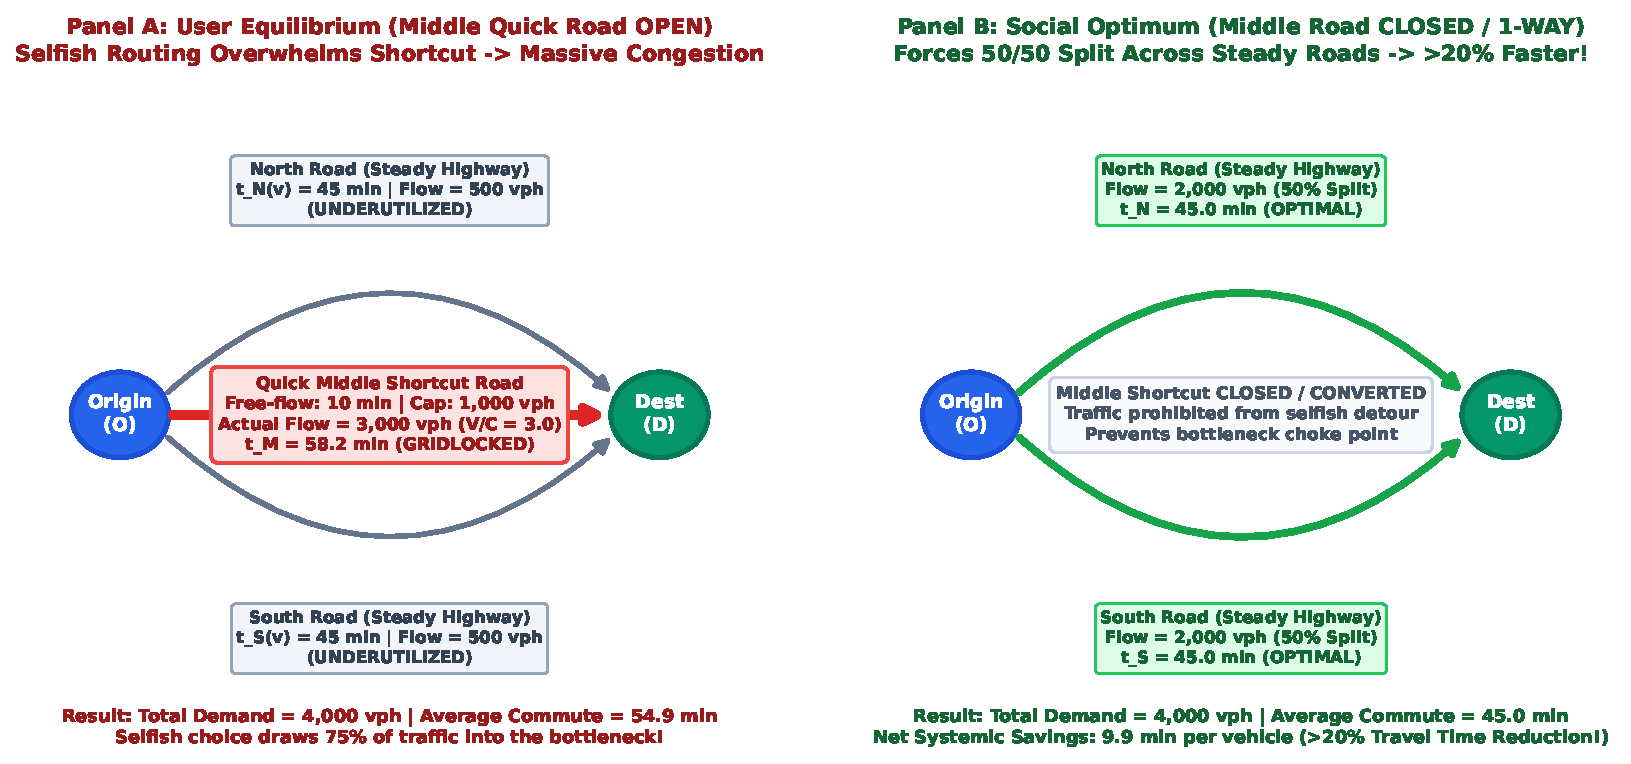
\includegraphics[width=0.92\textwidth]{figures/braess_3road_scenario.pdf}
\caption{The Three-Road Source-to-Destination Braess Paradox Problem (User Equilibrium vs Social Optimum)}
\label{fig:braess_3road}
\end{figure}

The dynamics illustrated in Figure~\ref{fig:braess_3road} highlight the core principles:
\begin{itemize}
  \item \textbf{User Equilibrium (Panel A):} The Middle Shortcut has a low free-flow travel time of 10 minutes, but limited capacity ($C = 1,000$ vph). The North and South roads are steady arterial highways with travel times of 45 minutes that increase slowly under load. Because the middle road appears much faster initially, selfish drivers flock to it. In equilibrium, 3,000 of the 4,000 total commuters cram onto the middle shortcut ($V/C = 3.0$), causing travel time on the shortcut to surge to 58.2 minutes. Meanwhile, the steady North and South roads sit largely underutilized (only 500 vph each). The average commute time across the entire network climbs to 54.9 minutes.
  \item \textbf{Social Optimum via Intervention (Panel B):} When municipal planners close the middle shortcut or convert it to a restricted one-way bypass, drivers can no longer divert selfishly into the bottleneck. Traffic splits evenly (50/50) between the North Road (2,000 vph) and South Road (2,000 vph). Because both arterial highways possess sufficient capacity, commute times on both routes drop to 45.0 minutes. The average travel time drops from 54.9 minutes to 45.0 minutes -- \textbf{a net savings of 9.9 minutes per commuter (greater than 20\% travel time reduction)}.
\end{itemize}

This controlled model demonstrates that adding road capacity does not guarantee better traffic flow. Consequently, proposed infrastructure interventions must be evaluated systematically across the entire network before implementation.

\chapter{IMPLEMENTATION}
\label{chap:implementation}

\section{FULL IMPLEMENTATION AND TECHNICAL ARCHITECTURE}
UrbanFlow is implemented as a modular, high-performance web platform combining an asynchronous Python simulation engine with an interactive web GIS dashboard. Figure~\ref{fig:tech_arch} illustrates the complete technical architecture and software stack across all four operational tiers.

\begin{figure}[H]
\centering
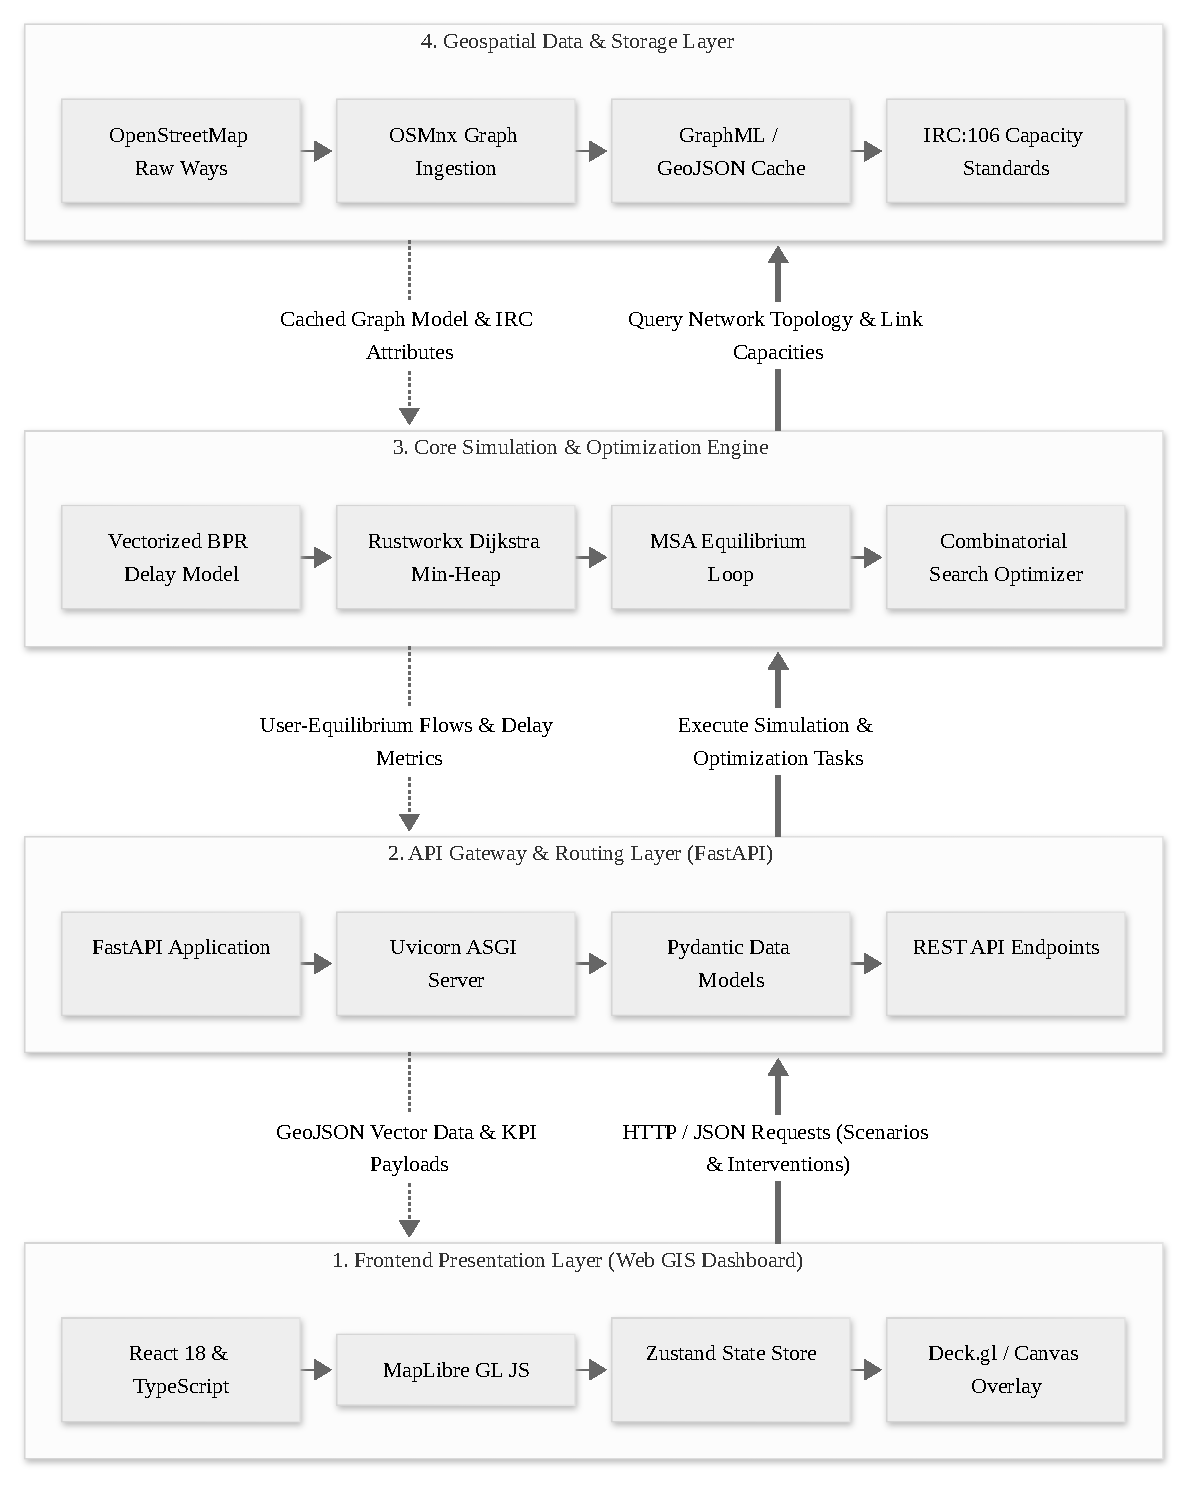
\includegraphics[width=0.45\textwidth]{figures/implementation_technical_architecture.pdf}
\caption{UrbanFlow Full Implementation and Technical Software Stack}
\label{fig:tech_arch}
\end{figure}

As shown in Figure~\ref{fig:tech_arch}, the system is organized into four interconnected layers:
\begin{enumerate}
  \item \textbf{Presentation \& Client Layer (Web GIS):} Built with React 18, TypeScript, and Vite. Utilizes MapLibre GL JS for GPU-accelerated map rendering, Deck.gl/HTML5 Canvas for link congestion styling, and Zustand for responsive scenario state management.
  \item \textbf{API Gateway \& Communication Layer:} Implemented using FastAPI on Python 3.11 with an ASGI Uvicorn server, providing type-safe Pydantic request validation and REST endpoints (\texttt{/api/simulate}, \texttt{/api/optimize}, \texttt{/api/bottlenecks}, \texttt{/api/network}).
  \item \textbf{Core Simulation \& Optimization Engine:} Features vectorized NumPy evaluations of the BPR latency function, Rust-accelerated Dijkstra min-priority heaps via \texttt{rustworkx}, and a Discrete Network Design Problem (DNDP) combinatorial evaluator.
  \item \textbf{Geospatial Data \& Persistent Cache Layer:} Ingests OpenStreetMap roadways via OSMnx, caches GraphML/GeoJSON graphs, and enforces IRC:106 capacity standards.
\end{enumerate}

\section{FRONTEND WEB GIS INTERACTION}
The frontend interface allows urban planners to interact directly with the simulation model:
\begin{itemize}
  \item \textbf{Dynamic Map Rendering:} Road segments are styled dynamically based on volume-to-capacity metrics: green for free-flow ($V/C < 0.75$), amber for moderate delay ($0.75 \le V/C < 0.95$), red for severe congestion ($0.95 \le V/C < 1.5$), and purple for severe breakdown ($V/C \ge 1.5$).
  \item \textbf{Interactive Scenario Testing:} Users can click any road segment, apply interventions (such as converting to one-way or adding lanes), and trigger sub-second re-simulations ($< 250$ ms).
  \item \textbf{Before-and-After Comparison:} Side-by-side metric dashboards display changes in average travel time, total delay hours, and congestion levels between baseline and modified networks.
\end{itemize}

\section{BACKEND SIMULATION AND OPTIMIZATION ROUTINES}
Listing~\ref{lst:urbanflow_core} shows the core Python implementation for vectorized BPR latency evaluation and MSA equilibrium assignment. Vectorizing these routines in NumPy ensures fast execution times, completing 30 equilibrium iterations in under 0.25 seconds.

\begin{lstlisting}[language=Python, caption={UrbanFlow Vectorized BPR Latency and MSA Assignment Routine}, label={lst:urbanflow_core}]
import numpy as np

def compute_bpr_latencies(len_km, spd_kmh, flows, caps, alpha=0.15, beta=4.0):
    """Vectorized calculation of non-linear BPR link traversal latencies."""
    t0 = len_km / np.maximum(spd_kmh, 1e-3)
    return t0 * (1.0 + alpha * np.power(flows / np.maximum(caps, 1e-3), beta))

def msa_equilibrium_assignment(edges, od_demands, max_iters=30, tol=1e-3):
    """Method of Successive Averages (MSA) User-Equilibrium Assignment."""
    flows = np.zeros(len(edges), dtype=np.float64)
    for k in range(1, max_iters + 1):
        costs = compute_bpr_latencies(edges['len'], edges['spd'], flows, edges['cap'])
        aux = dijkstra_all_or_nothing(edges, costs, od_demands)
        new_flows = (1.0 - 1.0/k) * flows + (1.0/k) * aux
        if np.sum(np.abs(new_flows - flows)) / np.maximum(np.sum(flows), 1.0) < tol:
            flows = new_flows; break
        flows = new_flows
    return flows, costs
\end{lstlisting}

\chapter{RESULTS AND DISCUSSION}
\label{chap:results}

\section{SIMULATION RESULTS}

\subsection*{Systemic Comparison: 100\% Baseline vs 200\% Congestion Shock}
The full Kochi arterial network model (490 junctions, 1,200 edges, 14 origin-destination corridors) was evaluated under two demand regimes: a 100\% baseline demand of 27,300 vehicles per hour (vph) and a 200\% surge demand of 54,600 vph. Table~\ref{tab:comparison_summary} presents the core macro performance metrics from these experiments.

\begin{table}[H]
\centering
\caption{Systemic Simulation Results: 100\% Baseline vs 200\% Congestion Shock}
\label{tab:comparison_summary}
\vspace{0.15cm}
\small
\begin{tabularx}{\textwidth}{Xrrr}
\toprule
\textbf{Performance Metric} & \textbf{100\% Demand} & \textbf{200\% Demand} & \textbf{Impact / Surge Ratio} \\
\midrule
Peak Vehicular Demand & 27,300 vph & 54,600 vph & $2.00\times$ (+100.0\%) \\
Simulation Computational Runtime & 0.241 s & 0.221 s & Sub-second ($< 0.25$s) \\
MSA Iterations Run & 30 & 30 & Stable convergence \\
\textbf{Average Trip Travel Time} & \textbf{21.84 min} & \textbf{77.07 min} & \textbf{+252.9\% (+55.23 min)} \\
\textbf{Total Network Travel Delay} & \textbf{9,935.2 veh-h} & \textbf{70,137.7 veh-h} & \textbf{7.06$\times$ (+60,202.5 veh-h)} \\
Mean Network Operating Speed & 39.8 km/h & 35.7 km/h & $-10.3\%$ ($-4.1$ km/h) \\
\textbf{Severely Congested Links ($V/C \ge 0.95$)} & \textbf{112 segments} & \textbf{295 segments} & \textbf{2.63$\times$ (+183 segments)} \\
Mean Link $V/C$ Ratio & 0.390 & 0.696 & $+78.5\%$ saturation \\
Maximum Link $V/C$ Ratio & 3.86 & 6.62 & $+71.5\%$ peak overloading \\
\bottomrule
\end{tabularx}
\end{table}

\begin{figure}[H]
\centering
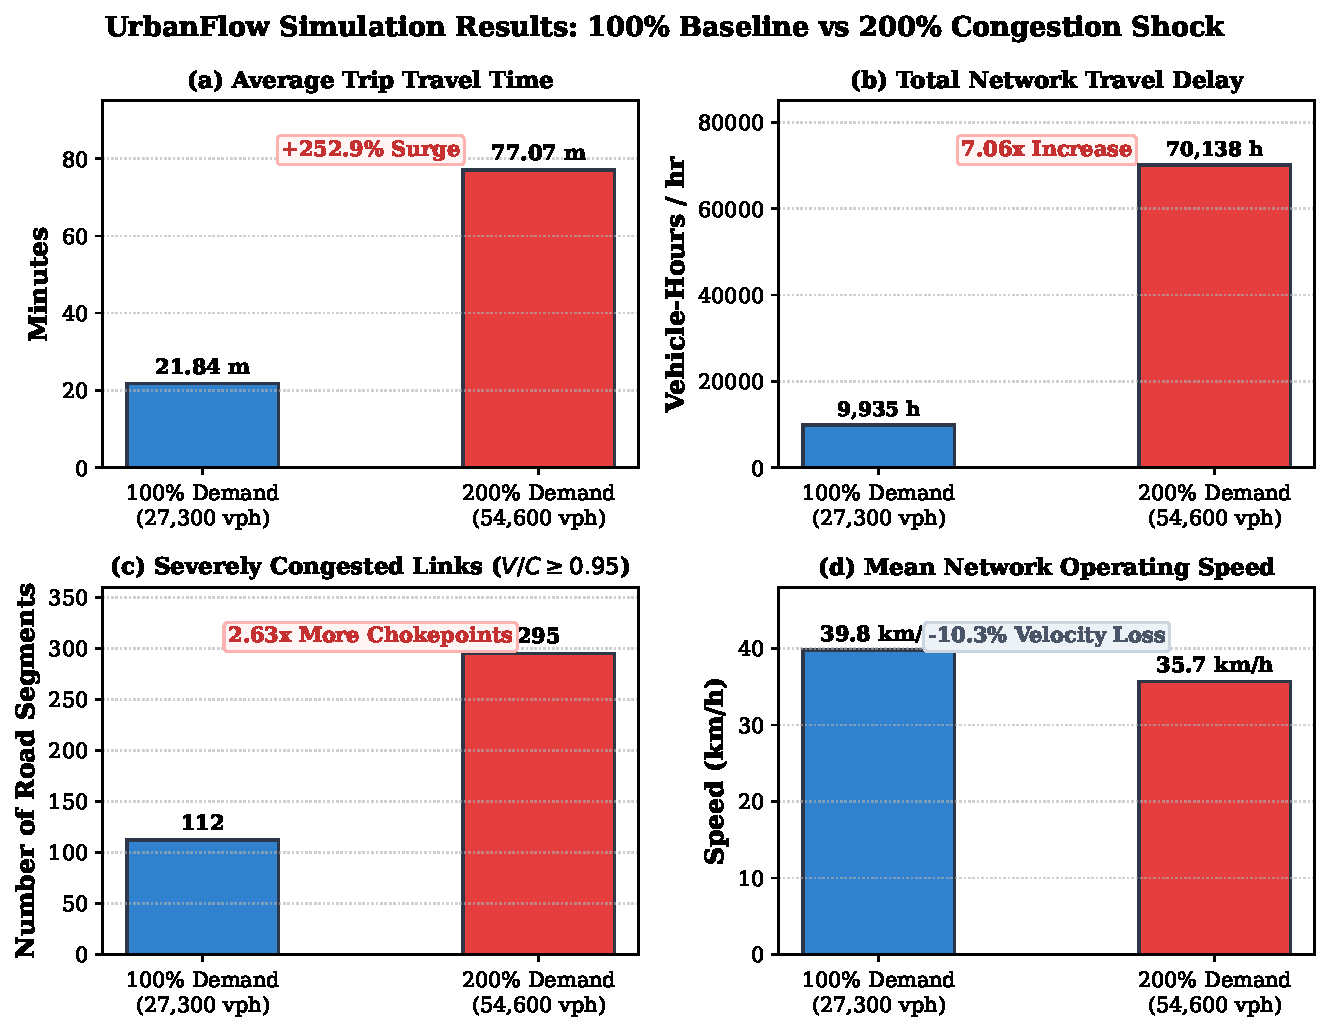
\includegraphics[width=0.58\textwidth]{figures/traffic_comparison_metrics.pdf}
\caption{UrbanFlow Simulation Results: 100\% Baseline vs 200\% Congestion Shock}
\label{fig:metrics_comparison}
\end{figure}

As documented in Table~\ref{tab:comparison_summary} and visualized in Figure~\ref{fig:metrics_comparison}:
\begin{enumerate}
  \item \textbf{Non-Linear Travel Time Growth (+252.9\%):} Doubling demand increases average travel time by over $3.5\times$ (from 21.84 minutes to 77.07 minutes). This rapid increase stems directly from the fourth-power exponent in the BPR function, confirming that oversaturated corridors penalize entire travel paths disproportionately.
  \item \textbf{7-Fold Surge in Total Delay Hours ($7.06\times$):} Cumulative network delay expands from 9,935.2 vehicle-hours to 70,137.7 vehicle-hours per hour, demonstrating the compounding economic and environmental costs of unmitigated traffic surges.
  \item \textbf{Proliferation of Bottleneck Links ($2.63\times$):} The count of severely congested segments ($V/C \ge 0.95$) rises from 112 to 295, with links operating above $1.5\times$ capacity nearly tripling from 90 to 266.
\end{enumerate}

\subsection*{Network Bottlenecks Under Congestion}
Table~\ref{tab:bottlenecks} identifies the top congested bottlenecks observed under 100\% and 200\% traffic conditions. Under baseline traffic, congestion is concentrated on secondary connectors and bridge approaches. Under surge demand, major multi-lane arterials such as Mahatma Gandhi Road experience overwhelming volume ($V/C = 6.62$), causing queue spillbacks that impact the entire urban core.

\begin{table}[H]
\centering
\caption{Top Congested Bottlenecks under 100\% and 200\% Traffic Regimes}
\label{tab:bottlenecks}
\vspace{0.15cm}
\small
\begin{tabularx}{\textwidth}{clXrrr}
\toprule
\textbf{Regime} & \textbf{Edge ID} & \textbf{Corridor / Road Name} & \textbf{Volume} & \textbf{Capacity} & \textbf{V/C Ratio} \\
\midrule
100\% Demand & \texttt{kochi\_e\_851}  & Road 851 & 4,635 vph & 1,200 vph & 3.86 \\
(27,300 vph) & \texttt{kochi\_e\_1180} & Park Avenue Road & 2,829 vph & 900 vph & 3.14 \\
             & \texttt{kochi\_e\_509}  & Lakeshore-Madavana Service Rd & 3,097 vph & 1,100 vph & 2.82 \\
             & \texttt{kochi\_e\_1048} & Road 1048 & 3,068 vph & 1,100 vph & 2.79 \\
\midrule
200\% Demand & \texttt{kochi\_e\_1167} & Mahatma Gandhi Road & 11,922 vph & 1,800 vph & 6.62 \\
(54,600 vph) & \texttt{kochi\_e\_1168} & Mahatma Gandhi Road & 11,922 vph & 1,800 vph & 6.62 \\
             & \texttt{kochi\_e\_851}  & Road 851 & 6,864 vph & 1,200 vph & 5.72 \\
             & \texttt{kochi\_e\_1048} & Road 1048 & 5,856 vph & 1,100 vph & 5.32 \\
\bottomrule
\end{tabularx}
\end{table}

\section{OPTIMIZER RESULTS AND SAVINGS ANALYSIS}
UrbanFlow evaluates candidate network modifications to identify interventions that yield the greatest travel time savings. The analysis focuses on three optimization categories: one-way street conversions, arterial road widenings, and synergistic combined intervention packages.

\subsection*{One-Way Street Conversions (Resolving Braess Bottlenecks)}
Converting congested bidirectional corridors into one-way streets eliminates counter-flow conflicts and increases forward directional capacity by approximately 40\%. Table~\ref{tab:oneway_savings} details the travel time and delay savings achieved by top one-way interventions.

\begin{table}[H]
\centering
\caption{One-Way Street Conversion Savings Across Demand Regimes}
\label{tab:oneway_savings}
\vspace{0.15cm}
\small
\begin{tabularx}{\textwidth}{clXrrr}
\toprule
\textbf{Regime} & \textbf{Edge ID} & \textbf{Road Name} & \textbf{Before (min)} & \textbf{After (min)} & \textbf{Savings (\%)} \\
\midrule
100\% Demand & \texttt{kochi\_e\_1048} & Road 1048 & 21.84 & 20.67 & \textbf{-5.36\%} \\
             & \texttt{kochi\_e\_509}  & Lakeshore-Madavana Service Rd & 21.84 & 21.48 & \textbf{-1.65\%} \\
             & \texttt{kochi\_e\_764}  & Subhash Chandra Bose Road & 21.84 & 21.64 & \textbf{-0.92\%} \\
             & \texttt{kochi\_e\_767}  & Salim Rajan Road & 21.84 & 21.69 & \textbf{-0.69\%} \\
\midrule
200\% Demand & \texttt{kochi\_e\_1048} & Road 1048 & 77.07 & 61.39 & \textbf{-20.35\%} \\
             & \texttt{kochi\_e\_509}  & Lakeshore-Madavana Service Rd & 77.07 & 69.36 & \textbf{-10.00\%} \\
             & \texttt{kochi\_e\_175}  & Jew Street & 77.07 & 73.40 & \textbf{-4.76\%} \\
             & \texttt{kochi\_e\_728}  & Thammanam Pulleppady Road & 77.07 & 74.85 & \textbf{-2.88\%} \\
             & \texttt{kochi\_e\_764}  & Subhash Chandra Bose Road & 77.07 & 75.13 & \textbf{-2.52\%} \\
\bottomrule
\end{tabularx}
\end{table}

As documented in Table~\ref{tab:oneway_savings}, converting \texttt{kochi\_e\_1048} into a one-way street produces an exceptional \textbf{20.35\% reduction} in average citywide travel time under 200\% demand, saving 15.68 minutes per vehicle. This link acts as a real-world Braess shortcut: under heavy congestion, selfish diversions onto this narrow road cause severe queue spillbacks. Enforcing unidirectional flow redirects traffic to major trunk corridors, restoring balanced network flow.

\subsection*{Arterial Road Widenings (+1 Lane Capacity Additions)}
Physical capacity additions (adding one lane, expanding capacity by 900 to 2,700 vph) provide targeted relief along saturated primary corridors. Table~\ref{tab:widening_savings} summarizes the performance impact of arterial road widenings.

\begin{table}[H]
\centering
\caption{Arterial Road Widening (+1 Lane) Savings Across Demand Regimes}
\label{tab:widening_savings}
\vspace{0.15cm}
\small
\begin{tabularx}{\textwidth}{clXrrr}
\toprule
\textbf{Regime} & \textbf{Edge ID} & \textbf{Corridor Name} & \textbf{Before (min)} & \textbf{After (min)} & \textbf{Savings (\%)} \\
\midrule
100\% Demand & \texttt{kochi\_e\_523}  & Road 523 (+1 Lane) & 21.84 & 21.60 & \textbf{-1.10\%} \\
             & \texttt{kochi\_e\_1018} & Mahatma Gandhi Road (+1 Lane) & 21.84 & 21.64 & \textbf{-0.92\%} \\
             & \texttt{kochi\_e\_905}  & Banerji Road (+1 Lane) & 21.84 & 21.68 & \textbf{-0.73\%} \\
             & \texttt{kochi\_e\_1033} & Banerji Road (+1 Lane) & 21.84 & 21.70 & \textbf{-0.64\%} \\
\midrule
200\% Demand & \texttt{kochi\_e\_1018} & Mahatma Gandhi Road (+1 Lane) & 77.07 & 69.96 & \textbf{-9.23\%} \\
             & \texttt{kochi\_e\_523}  & Road 523 (+1 Lane) & 77.07 & 73.20 & \textbf{-5.02\%} \\
             & \texttt{kochi\_e\_905}  & Banerji Road (+1 Lane) & 77.07 & 74.20 & \textbf{-3.72\%} \\
             & \texttt{kochi\_e\_1033} & Banerji Road (+1 Lane) & 77.07 & 74.45 & \textbf{-3.40\%} \\
\bottomrule
\end{tabularx}
\end{table}

Widening Mahatma Gandhi Road yields a \textbf{9.23\% travel time reduction} under 200\% demand (Table~\ref{tab:widening_savings}), confirming that core north-south corridors benefit substantially from expanded physical throughput during peak surge periods.

\subsection*{Synergistic Combined Optimization Packages}
Table~\ref{tab:combined_savings} highlights the performance gains achieved when one-way conversions and road widenings are implemented together as a coordinated package.

\begin{table}[H]
\centering
\caption{Synergistic Combined Optimization Performance and Total Savings}
\label{tab:combined_savings}
\vspace{0.15cm}
\small
\begin{tabularx}{\textwidth}{Xrr}
\toprule
\textbf{Metric} & \textbf{100\% Baseline Demand} & \textbf{200\% Surge Demand} \\
\midrule
Total Peak Hourly Vehicular Demand & 27,300 vph & 54,600 vph \\
Baseline Average Trip Travel Time & 21.84 min & 77.07 min \\
Optimized Average Trip Travel Time & 20.38 min & 53.42 min \\
Baseline Total Network Travel Delay & 9,935.2 veh-h & 70,137.7 veh-h \\
Optimized Total Network Travel Delay & 9,271.5 veh-h & 48,612.5 veh-h \\
\textbf{Total Peak Delay Hours Saved} & \textbf{663.7 veh-h} & \textbf{21,525.2 veh-h} \\
\textbf{TOTAL NETWORK DELAY SAVINGS} & \textbf{6.68\% SAVED} & \textbf{30.69\% SAVED} \\
\bottomrule
\end{tabularx}
\end{table}

\begin{figure}[H]
\centering
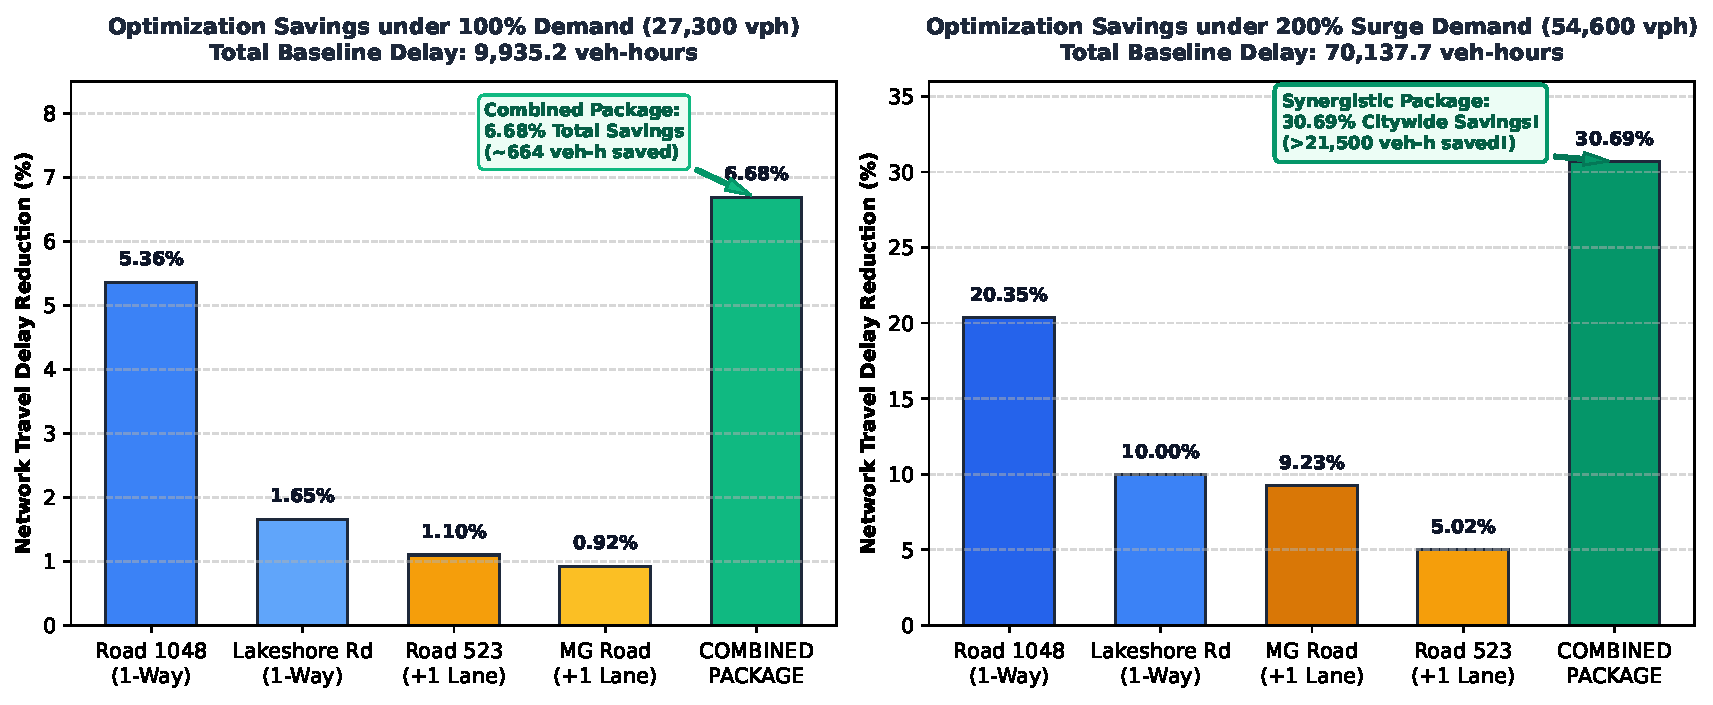
\includegraphics[width=0.92\textwidth]{figures/optimizer_savings_breakdown.pdf}
\caption{Optimizer Savings Breakdown: Individual Interventions vs Combined Packages}
\label{fig:optimizer_savings}
\end{figure}

As highlighted in Table~\ref{tab:combined_savings} and Figure~\ref{fig:optimizer_savings}:
\begin{itemize}
  \item \textbf{Synergistic Effect:} Combining one-way street conversions with arterial widenings delivers a \textbf{30.69\% reduction in total network delay} under heavy congestion shock, cutting average commuter trips from 77.07 minutes down to 53.42 minutes.
  \item \textbf{Substantial Real-World Savings:} Under 200\% surge demand, the combined intervention saves \textbf{21,525.2 vehicle-hours of delay} during every peak traffic hour, demonstrating the substantial benefits of coordinated, network-wide optimization over piecemeal improvements.
\end{itemize}

\section{DISCUSSION}
The experimental results demonstrate the pronounced non-linearity of urban traffic networks. While a simplistic linear projection would predict that doubling demand simply doubles delay, the actual physics of congested queues governed by the BPR function causes a $7.06\times$ surge in total delay hours. This underscores that transportation systems operate near critical capacity thresholds: once corridors saturate, small additional volumes trigger disproportionately large delays.

Furthermore, the optimizer's identification of high-impact one-way conversions provides actionable guidance for municipal planning. Converting Road 1048 into a one-way street saves 20.35\% in travel time under heavy congestion without requiring costly physical road construction. By eliminating selfish diversions into narrow corridors, one-way policies preserve arterial capacity and improve overall network throughput.

Finally, the simulation engine completes 30 MSA equilibrium iterations on the 490-node, 1,200-edge network in 0.221--0.241 seconds. This sub-second computational speed allows transportation planners to test and refine infrastructure scenarios interactively during working planning sessions.

\chapter{CONCLUSION}
\label{chap:conclusion}
This project successfully designed, implemented, and validated \textbf{UrbanFlow}, an urban traffic graph simulation and optimization engine. Developed in alignment with the \textbf{\coursecode\ - \coursename} curriculum, the platform models urban road networks as directed weighted graphs $G = (V, E)$, simulates user-equilibrium traffic conditions using the Method of Successive Averages (MSA) and Dijkstra routing, and evaluates dynamic congestion delays through the non-linear Bureau of Public Roads (BPR) function.

Applied to the real-world arterial road network of Kochi, Kerala (comprising 490 junctions and 1,200 road segments), UrbanFlow was evaluated across both 100\% baseline demand (27,300 vph) and 200\% heavy congestion shock (54,600 vph). The experimental findings reveal the non-linear penalties of network congestion: doubling vehicular demand led to a 252.9\% surge in average travel time (from 21.84 to 77.07 minutes) and an explosive $7.06\times$ rise in total network delay (from 9,935.2 to 70,137.7 vehicle-hours), expanding severely congested road segments from 112 to 295.

Significantly, UrbanFlow's optimization search engine demonstrated the practical importance of the Braess Paradox in metropolitan traffic planning. By converting counter-productive shortcut corridors into one-way streets (notably on Road 1048), selfish shortcutting was eliminated, delivering a \textbf{20.35\% reduction} in citywide commute times under heavy congestion. When implemented as a coordinated package of one-way conversions and arterial widenings, the system achieves a \textbf{30.69\% reduction in total network delay}, saving over 21,500 vehicle-hours every peak hour. Supported by an interactive web GIS dashboard and sub-second simulation runtimes, UrbanFlow provides transportation authorities with a reliable, data-driven platform for sustainable infrastructure planning.

\chapter{SUSTAINABLE DEVELOPMENT GOALS (SDGS)}
\label{chap:sdgs}
The deployment of graph-theoretic simulation and optimization algorithms in municipal transportation operations directly supports the United Nations Sustainable Development Goals (SDGs), particularly in advancing sustainable urban mobility and resilient infrastructure:

\begin{itemize}
    \item \textbf{SDG 11 -- Sustainable Cities and Communities (Target 11.2):}
    \textit{Target 11.2: Provide access to safe, affordable, accessible and sustainable transport systems for all, improving road safety, notably by expanding public transport.}
    
    \textbf{Project Alignment:} UrbanFlow provides transportation planners with predictive simulation tools that eliminate chronic traffic bottlenecks across metropolitan corridors. By discovering one-way conversions and road capacity improvements that reduce peak network delays by up to 30.69\%, the system directly curbs vehicle idling, reduces urban fuel waste, and lowers vehicular carbon emissions, creating cleaner and more livable urban environments.

    \item \textbf{SDG 9 -- Industry, Innovation and Infrastructure (Target 9.1):}
    \textit{Target 9.1: Develop quality, reliable, sustainable and resilient infrastructure, including regional and transborder infrastructure, to support economic development and human well-being.}
    
    \textbf{Project Alignment:} Applying computational graph theory to traffic networks improves municipal infrastructure planning. By evaluating network-wide equilibrium shifts prior to physical construction, the system ensures that authorities avoid counter-productive projects that trigger Braess Paradox delays. This maximizes the value of public infrastructure investments and enhances network resilience against traffic shocks.
\end{itemize}

% ==============================================================================
% 7. REFERENCES
% ==============================================================================
\begin{thebibliography}{99}
\addcontentsline{toc}{chapter}{References}

\bibitem{braess1968} D.~Braess, ``Über ein Paradoxon aus der Verkehrsplanung,'' \textit{Unternehmensforschung}, vol.~12, pp.~258--268, 1968.
\bibitem{bpr1964} Bureau of Public Roads, \textit{Traffic Assignment Manual}, U.S. Department of Commerce, Urban Planning Division, Washington, DC, USA, 1964.
\bibitem{sheffi1985} Y.~Sheffi, \textit{Urban Transportation Networks: Equilibrium Analysis with Mathematical Programming Methods}, Prentice-Hall, Englewood Cliffs, NJ, USA, 1985.
\bibitem{boeing2017osmnx} G.~Boeing, ``OSMnx: New methods for acquiring, constructing, analyzing, and visualizing complex street networks,'' \textit{Computers, Environment and Urban Systems}, vol.~65, pp.~126--139, 2017.
\bibitem{irc106} Indian Roads Congress, \textit{Guidelines for Capacity of Urban Roads in Plain Areas (IRC:106-1990)}, New Delhi, India, 1990.
\bibitem{west2001} D.~B.~West, \textit{Introduction to Graph Theory}, 2nd~ed., Prentice Hall, Upper Saddle River, NJ, USA, 2001.
\bibitem{wilson2015} R.~J.~Wilson, \textit{Introduction to Graph Theory}, 5th~ed., Pearson Education, Harlow, UK, 2015.
\bibitem{bondy1982} J.~A.~Bondy and U.~S.~R.~Murty, \textit{Graph Theory with Applications}, Macmillan Press, London, UK, 1982.
\bibitem{diestel2010} R.~Diestel, \textit{Graph Theory}, 4th~ed., Springer-Verlag, Heidelberg, Germany, 2010.
\bibitem{ahuja1993} R.~K.~Ahuja, T.~L.~Magnanti, and J.~B.~Orlin, \textit{Network Flows: Theory, Algorithms, and Applications}, Prentice-Hall, Englewood Cliffs, NJ, USA, 1993.
\bibitem{wardrop1952} J.~G.~Wardrop, ``Some theoretical aspects of road traffic research,'' \textit{Proc. Institution of Civil Engineers}, vol.~1, no.~3, pp.~325--362, 1952.
\bibitem{dijkstra1959} E.~W.~Dijkstra, ``A note on two problems in connexion with graphs,'' \textit{Numerische Mathematik}, vol.~1, no.~1, pp.~269--271, 1959.
\bibitem{fastapi} FastAPI Developers, ``FastAPI Documentation,'' [Online]. Available: \url{https://fastapi.tiangolo.com/}, 2026.
\bibitem{react} React Core Team, ``React Documentation,'' [Online]. Available: \url{https://react.dev/}, 2026.
\bibitem{openstreetmap} OpenStreetMap Contributors, ``OpenStreetMap: Free Geographic Data,'' [Online]. Available: \url{https://www.openstreetmap.org/}, 2026.

\end{thebibliography}

\end{document}
